\documentclass[logo,reportComp]{thesis}
\usepackage[cpp,linenum]{mypackage}

\title{计算机图形学}
\subtitle{作业六:光照效果}
\school{数据科学与计算机学院}
\author{陈鸿峥}
\classname{17大数据与人工智能}
\stunum{17341015}
\headercontext{计算机图形学作业}

\begin{document}

\maketitle

\section{实验原理}

\section{实验结果}
双击\verb'teapot.exe'即可运行,实验结果如图\ref{fig:teapot}所示。
\begin{figure}[H]
\centering
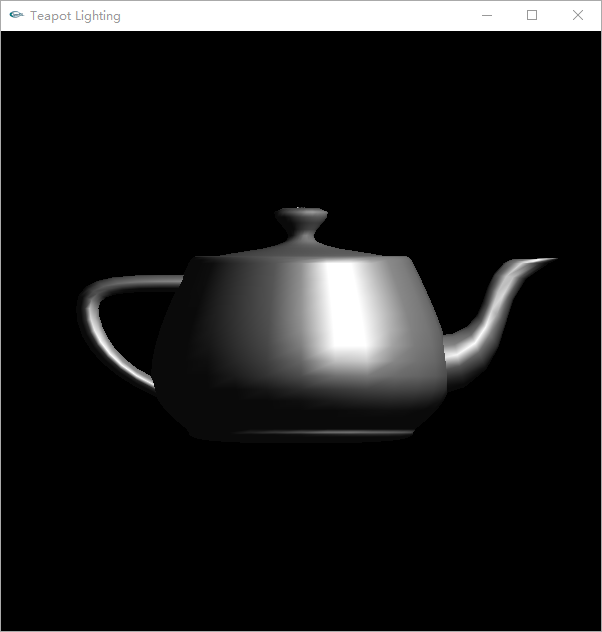
\includegraphics[width=0.6\linewidth]{fig/result.png}
\caption{Teapot光照结果}
\label{fig:teapot}
\end{figure}

\appendixconfig
\appendix
\section{源代码}
\lstinputlisting{teapot.c}

编译指令如下:
\begin{flushleft}
\verb'gcc -I.\include -L.\lib teapot.c -lglu32 -lglut32 -lopengl32 -o teapot.exe'
\end{flushleft}

\end{document}
% 题目: 用 OpenGL 实现简单的光照效果。
% 功能要求:
% 1. 显示默认的 Teapot 模型
% 2. 为 Teapot 模型建立 Smooth Shading 效果,如图 1 所示。
% 实现提示:
% 1. 利用 OpenGL 的 API 初始化 material property, light source, lighting model, depth buffer 等信息。
% 2. 使用 OpenGL Shader 实现。
% 3. 显示如下类似效果:

% 要求:
% 1. 作业按百分制评分, 没交作业算 0 分;
% 2. 提交代码文件,缺源代码文件的作业成绩减 10 分;
% 3. 提交直接可执行的程序文件或脚本文件,不能运行的程序(含出错,缺 dll 文件等) 作业成绩减 10 分;
% 4. 作业文档,包含简要的程序文件说明,运行方法,以及程序运行结果截图,缺文档的作业成绩减 10 分;
% 5. 发现作业抄袭的本次作业算 0 分。

% OpenGL(七) 光照模型及设置 https://blog.csdn.net/dcrmg/article/details/53121938
% http://what-when-how.com/opengl-programming-guide/creating-light-sources-opengl-programming/